\documentclass[preview,border=5pt]{standalone}
\usepackage{teaching}
\begin{document}

\centering
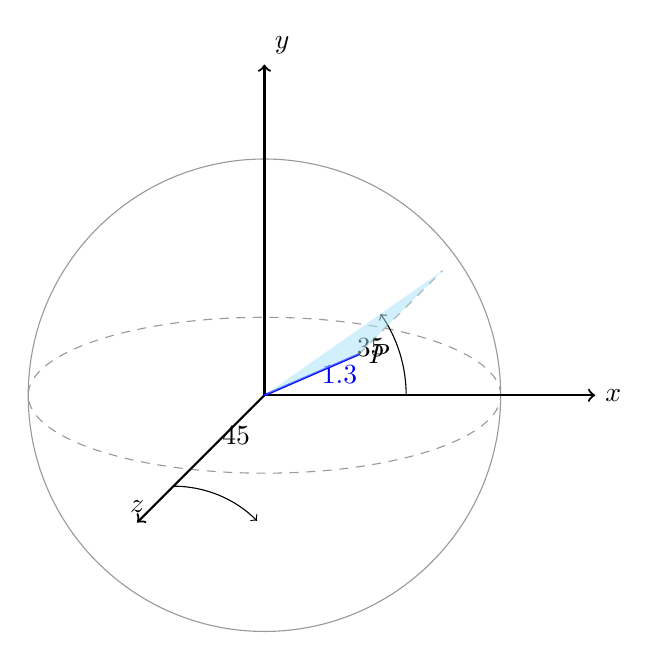
\begin{tikzpicture}[scale=3, line cap=round]

%---- STYLES ----
\tikzset{
    axis/.style={->, thick},
    rho/.style={blue, thick},
    proj/.style={gray!70, dashed},
}

% ORIGIN
\coordinate (O) at (0,0,0);

% POINT P in spherical coords
\def\rho{1.3}
\def\theta{35}   % azimuth (in xy-plane)
\def\phi{45}     % polar angle (from +z axis)

% Convert spherical → Cartesian
\pgfmathsetmacro{\Px}{\rho*sin(\phi)*cos(\theta)}
\pgfmathsetmacro{\Py}{\rho*sin(\phi)*sin(\theta)}
\pgfmathsetmacro{\Pz}{\rho*cos(\phi)}

\coordinate (P) at (\Px,\Py,\Pz);

% Projection onto xy-plane
\coordinate (Q) at (\Px,\Py,0);

%---- DRAW SPHERE ----
\draw[black!40] (0,0,0) circle (1);               % outline
\draw[black!40, dashed] (0,0,0) ellipse (1 and 0.33); % equatorial projection

%---- AXES ----
\draw[axis] (0,0,0) -- (0,0,1.4) node[above] {$z$};
\draw[axis] (0,0,0) -- (1.4,0,0) node[right] {$x$};
\draw[axis] (0,0,0) -- (0,1.4,0) node[above right] {$y$};

%---- RADIUS ----
\draw[rho] (O) -- (P) node[midway, right] {$\rho$};

% Vertical from P to xy-plane
\draw[proj] (P) -- (Q);

%--- POINT LABELS
\node[right] at (P) {$P$};

%--- ANGLE φ (vertical)
\draw[->] (0,0,1) arc[start angle=90, end angle=90-\phi, radius=0.5];
\node at (0.15,0.1,0.7) {$\phi$};

%--- ANGLE θ (azimuth)
\draw[->] (0.6,0,0) arc[start angle=0, end angle=\theta, radius=0.6];
\node at (0.45,0.2,0) {$\theta$};

%--- Shaded projection triangle
\fill[cyan!35, opacity=0.5]
    (0,0,0) -- (Q) -- (P) -- cycle;

\end{tikzpicture}

\end{document}